\documentclass[a4paper,11pt]{article}
\usepackage[fontset=fandol]{ctex}
\usepackage[margin=2cm]{geometry}
\usepackage{amsmath,amssymb,mathtools}
\usepackage{booktabs,longtable,array}
\usepackage{enumitem}
\usepackage{graphicx}
\usepackage{hyperref}
\usepackage{float}
\usepackage{caption}

\setlength{\parindent}{0pt}
\setlength{\parskip}{0.45em}
\hypersetup{colorlinks=true,linkcolor=blue,urlcolor=blue}
\graphicspath{{./}{./figures/}}

\title{UCB CS294/194-196 Agentic AI Fall 2025\\第09讲：AI Agents to Automate Scientific Discoveries}
\author{基于公开视频、字幕、课程页与官方 readings 整理}
\date{}

\begin{document}
\maketitle
\tableofcontents
\newpage

\section{为什么科学发现会成为 agentic AI 的高价值场景}
James Zou 这一讲的起点非常清晰：科学研究本身就是一个闭环过程，包含假设提出、文献检索、实验设计、工具调用、结果分析、复验与迭代。LLM agent 之所以适合科学发现，不是因为它们天然“聪明”，而是因为科学工作本来就高度依赖结构化协作、工具链调用和长时间尺度上的累积。 

从课程视频和官方 readings 的共同信息来看，最有前景的路径不是让单个大模型包办全部科研工作，而是让多个角色化 agent 共同参与：有人负责方向判断，有人负责文献浏览，有人负责实验设计，有人负责数据分析，还有人负责挑错与复核。人类研究者则继续承担高层约束、伦理边界、方向筛选和最终判断。

\begin{figure}[H]
  \centering
  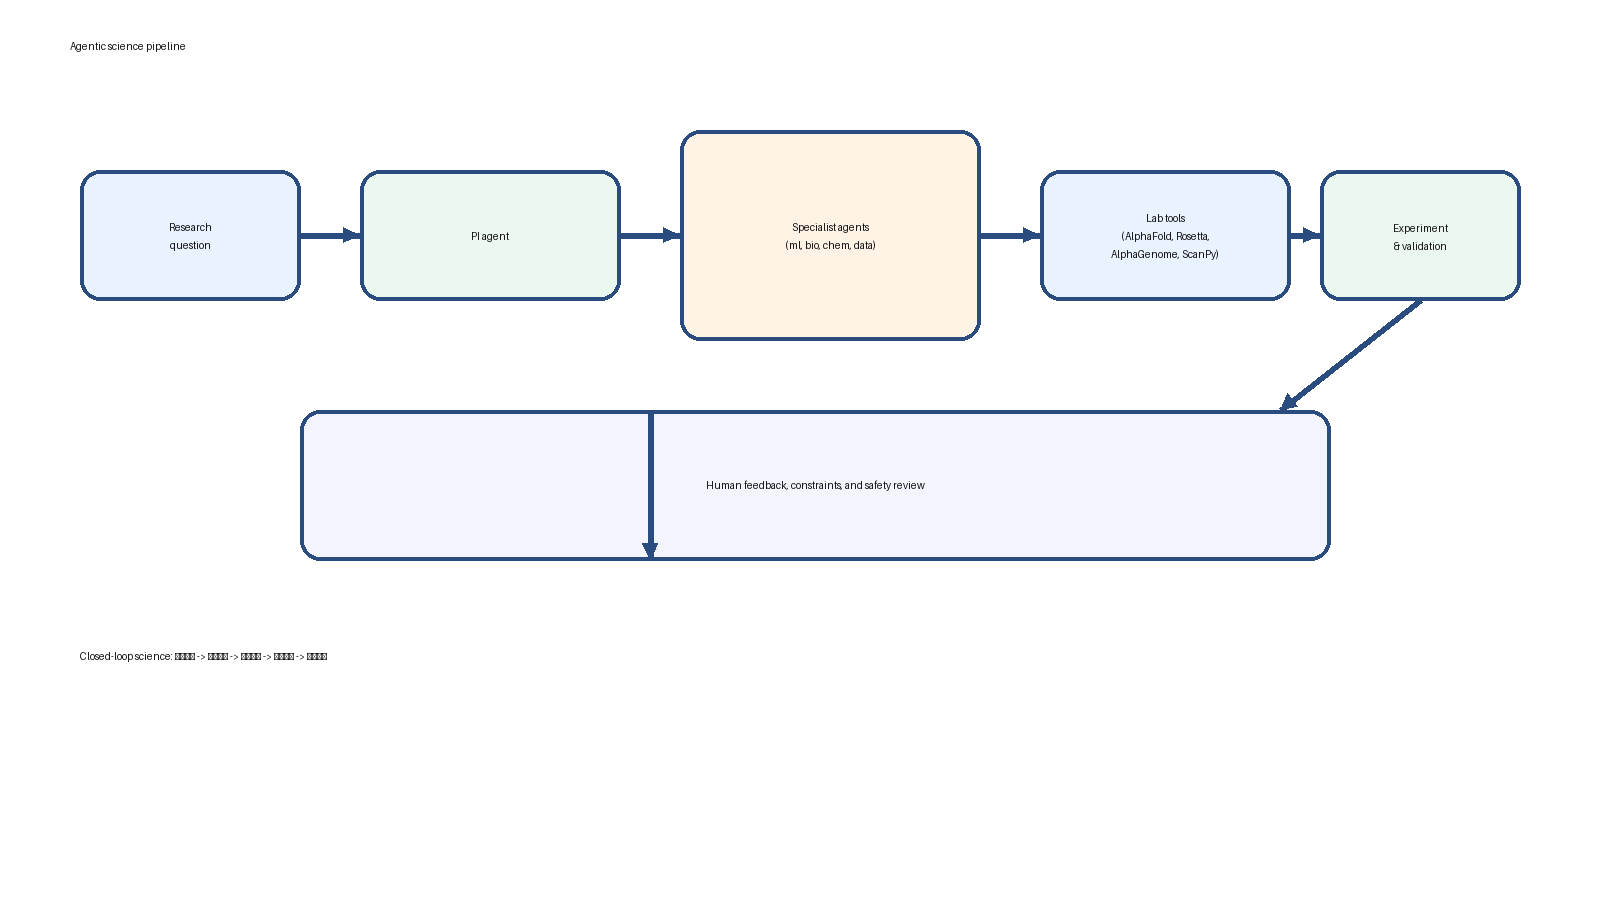
\includegraphics[width=0.94\linewidth]{figures/agentic_science_pipeline.png}
  \caption{本讲的总括图：科学发现可以被看作“目标定义 -> 专家分工 -> 工具执行 -> 结果验证 -> 人类反馈”的闭环系统。}
\end{figure}

\section{Virtual Lab：把研究组织成一组可协作的 agents}
课程中最有代表性的系统是 Virtual Lab。它不是一个单一聊天助手，而是一个由多个 LLM scientist agents 构成的研究组织。核心角色包括：
\begin{itemize}[leftmargin=1.4em]
  \item \textbf{PI agent}：像 principal investigator 一样负责目标分配、课题筛选和会议调度。
  \item \textbf{student agents}：承担具体子任务，例如文献阅读、实验方案草拟、数据处理或工具调用。
  \item \textbf{teacher agents}：提供更系统化的训练任务和反馈，让 student agents 学会特定技能。
  \item \textbf{critic agent}：专门挑错、找漏洞、提出替代解释。
  \item \textbf{memory / sandbox}：让 agents 能记录上下文、保存中间结果，并在受控环境里调用外部工具。
\end{itemize}

这套组织的关键不是“每个 agent 都很强”，而是它们在制度上分工明确。PI agent 不需要自己知道所有细节；它只要知道何时该调用什么专家、何时该做汇总、何时该回到人类确认即可。教师 agent 的作用是把研究任务拆成训练问题；critic agent 的作用是防止系统在长链路里漂移。课程强调，这类结构特别适合科学任务，因为科学本身就是跨领域协作，而不是单一推理轨迹。

\begin{figure}[H]
  \centering
  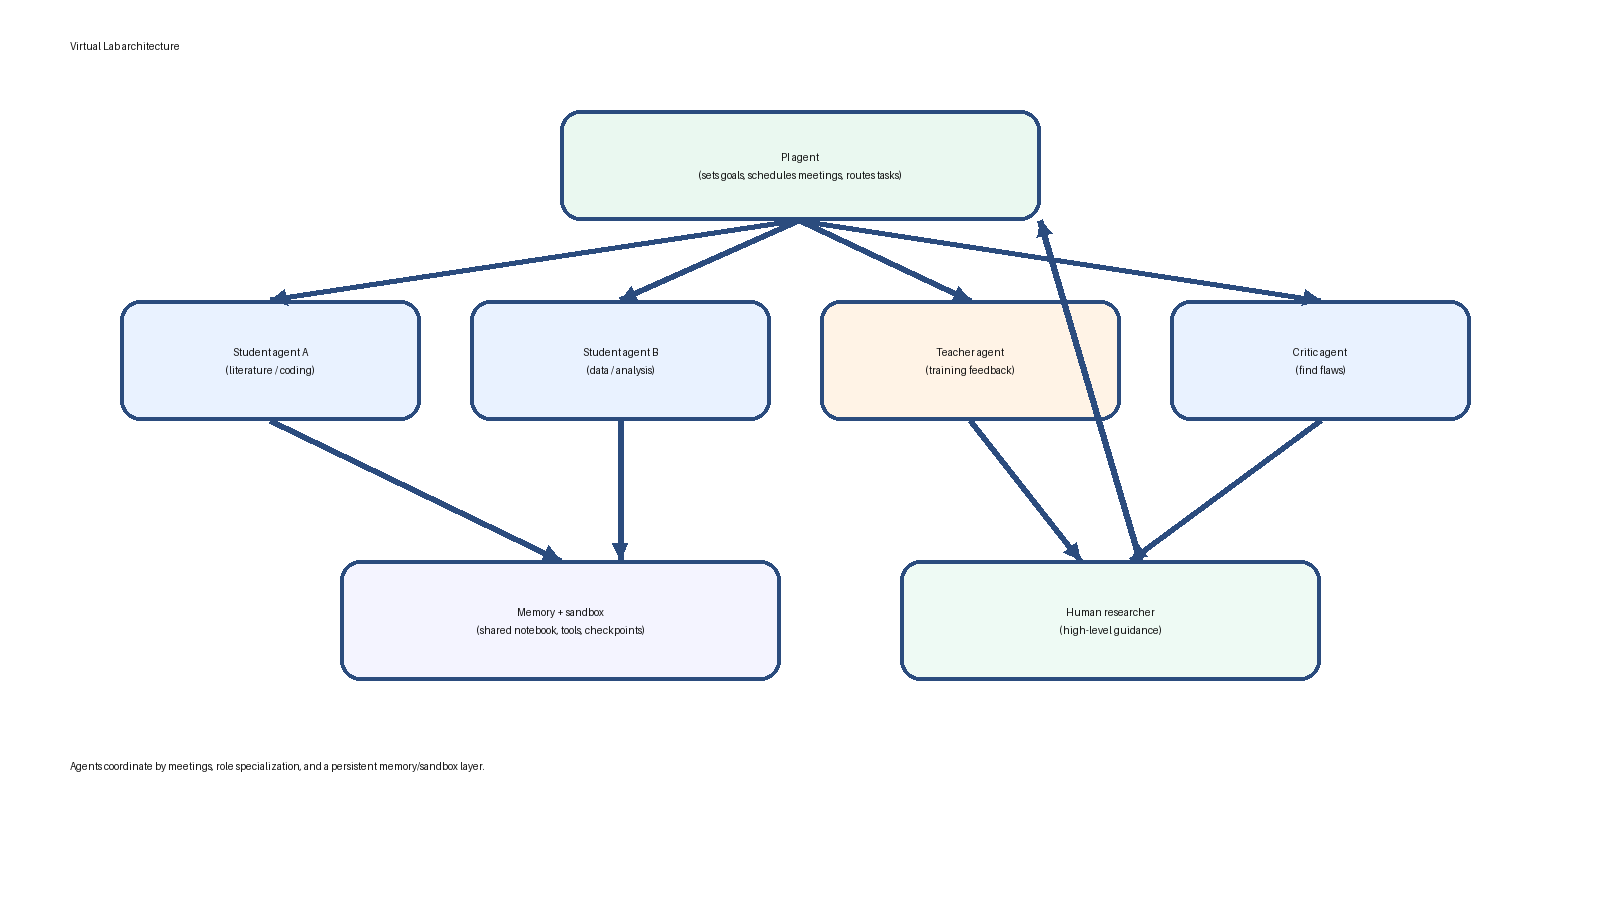
\includegraphics[width=0.94\linewidth]{figures/virtual_lab_architecture.png}
  \caption{Virtual Lab 的组织方式：PI agent 统筹，专长 agent 执行，critic agent 挑错，memory 与 sandbox 维持长期研究状态。}
\end{figure}

\section{案例一：Virtual Lab 如何设计 SARS-CoV-2 nanobodies}
官方 reading《The Virtual Lab of AI agents designs new SARS-CoV-2 nanobodies》给出了这套方法最有说服力的例子。系统不是凭空“生成一个分子”，而是沿着科学上真实可操作的管线推进。大致流程是：
\begin{enumerate}[leftmargin=1.6em]
  \item 设定研究目标：面向最近变异株设计可结合的 nanobody binders。
  \item 由 agent 生成候选序列，并对候选进行筛选。
  \item 用 AlphaFold-Multimer、Rosetta 和相关蛋白语言模型对结构与结合可能性做评估。
  \item 将保留下来的候选送往实验验证，观察其对不同变体的 binding profile。
  \item 结合实验结果继续修正筛选标准与设计策略。
\end{enumerate}

论文摘要明确给出几个关键事实：系统最终设计出 92 个新的 nanobodies；实验验证显示其中一些分子对 JN.1 或 KP.3 变体有更好的结合，同时仍保留对祖先 spike protein 的强结合；这说明 AI agents 不只是能“写计划”，而是能在真实实验闭环里推动发现。

\begin{figure}[H]
  \centering
  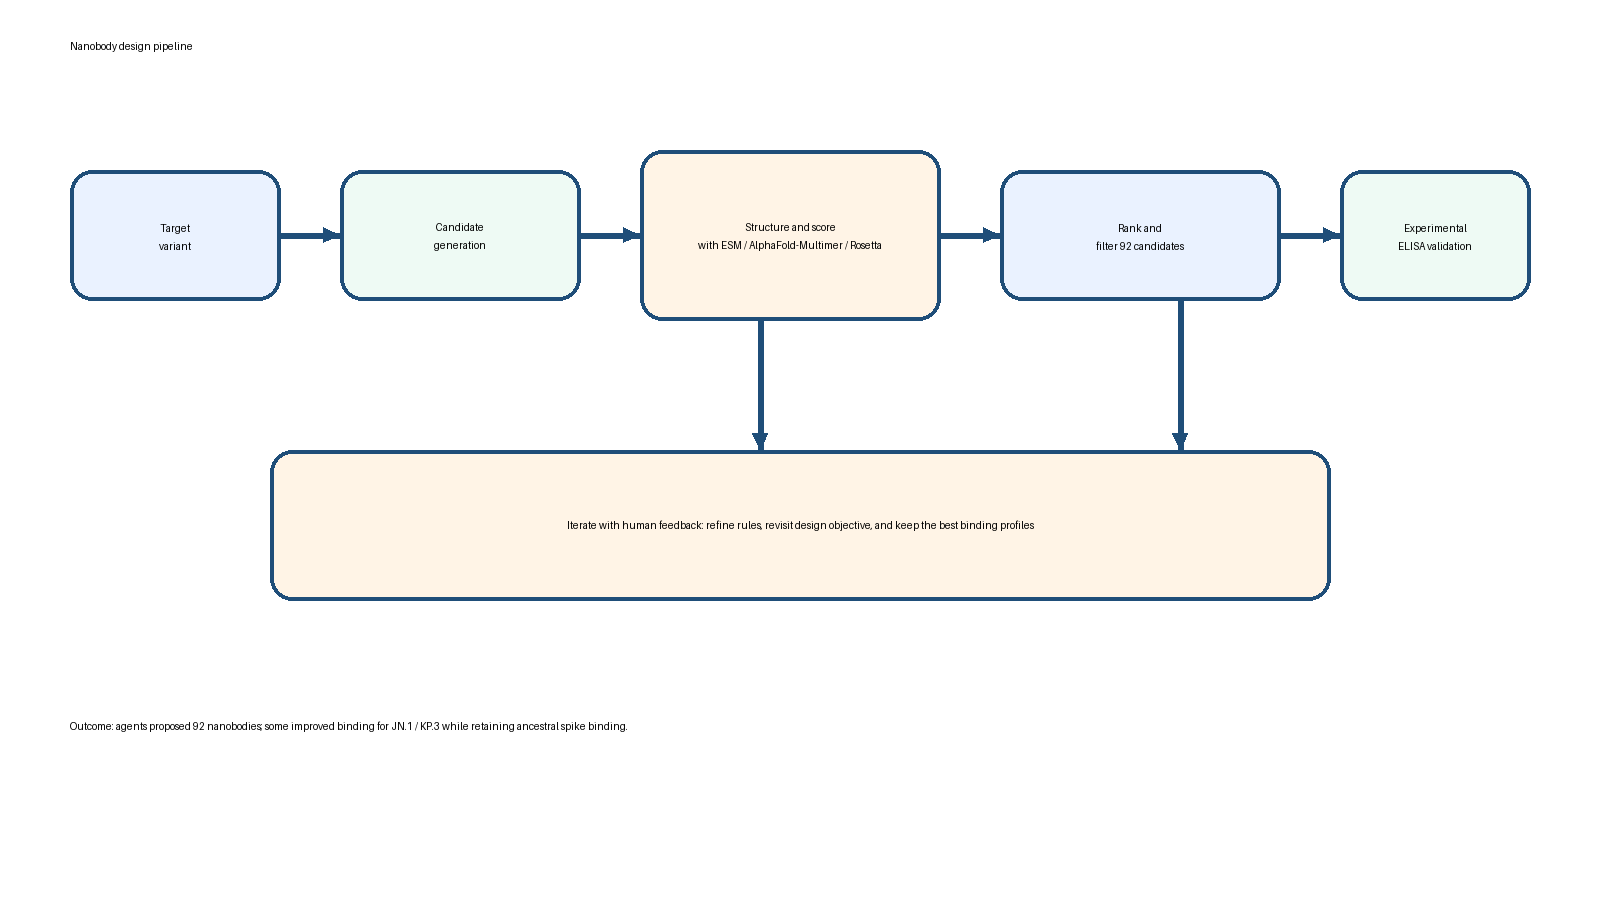
\includegraphics[width=0.94\linewidth]{figures/nanobody_pipeline.png}
  \caption{Nanobody 设计的 agentic pipeline：从目标定义、候选生成、结构评估到实验验证。}
\end{figure}

这一案例的重要性在于它展示了一种现实主义的自动化科学观：AI 并没有取消实验，也没有取消人类专家，而是把研究流程拆得更细，并把每一步的中间产物变成可复用的上下文。换句话说，agent 的价值不是替代实验，而是让实验之前的迭代成本大幅下降。

\section{案例二：Paper2Agent，把论文变成可交互的研究助手}
第二篇官方 reading《Paper2Agent: Reimagining Research Papers As Interactive and Reliable AI Agents》把课程主题推进了一步：不仅科学实验可以 agent 化，研究论文本身也可以被转化为 agent。这里的核心思想是把静态论文变成一个能回答问题、能调用工具、能复现结果的交互式系统。

Paper2Agent 的工作流非常清晰：
\begin{itemize}[leftmargin=1.4em]
  \item 多个 agent 分别分析论文文本和对应 codebase。
  \item 系统据此构建一个 Model Context Protocol（MCP）server，把论文的方法、数据与工具包装成可调用接口。
  \item 随后通过迭代测试不断修复和加固这个 paper agent，直到它既能复现论文结果，又能回答新的科研查询。
  \item 最后把该 MCP 接到聊天式 agent 上，例如 Claude Code，形成面向研究者的自然语言接口。
\end{itemize}

\begin{figure}[H]
  \centering
  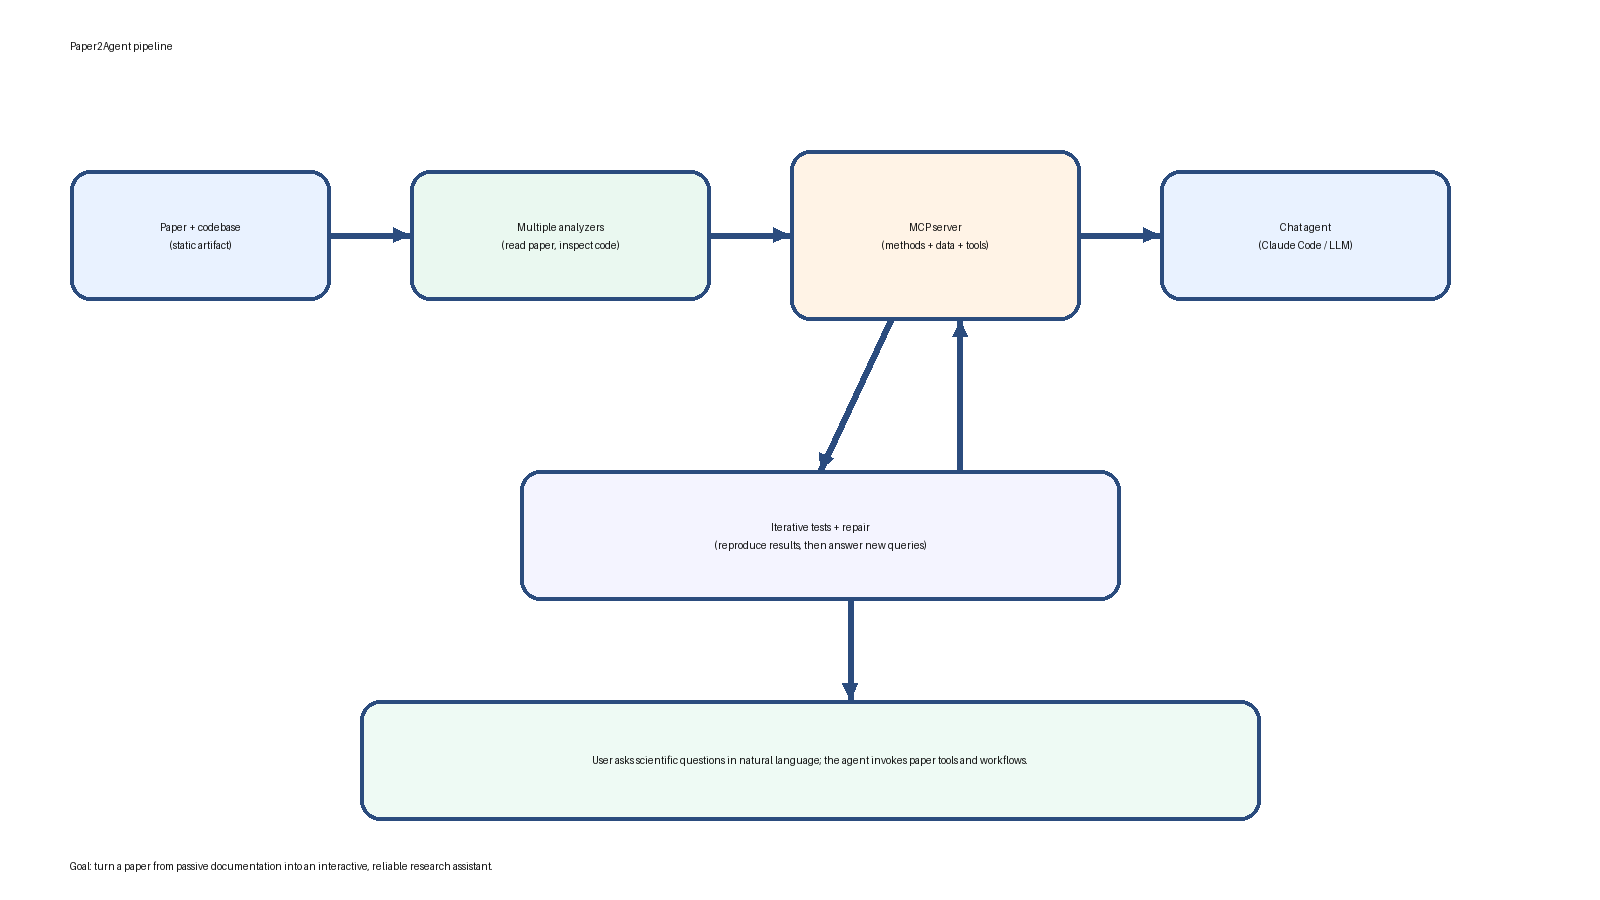
\includegraphics[width=0.94\linewidth]{figures/paper2agent_pipeline.png}
  \caption{Paper2Agent 的核心思想：把论文、代码和数据封装成一个可交互的 MCP 研究代理。}
\end{figure}

论文摘要中提到的案例包括 AlphaGenome、ScanPy 和 TISSUE。系统利用这些基础工具构建出分别用于基因变异解释、单细胞分析和空间转录组分析的 paper agents。课程视频里还特别提到，这类系统可以让两个 paper agent 直接进行 agent-to-agent collaboration，例如一个方法 agent 与一个数据 agent 直接协作，从而把跨论文的交互变成研究常态。

\section{这类系统到底解决了什么问题}
这讲不是在鼓吹“全自动科学”，而是在总结几个当前最现实的增益点。
\begin{enumerate}[leftmargin=1.6em]
  \item \textbf{把知识从静态文档变成可执行接口}：研究者不必手工翻论文、找代码入口、猜参数。
  \item \textbf{把长链路研究拆成可审计步骤}：每个 agent 的输出都可以被记录、回放和复核。
  \item \textbf{把专业分工显式化}：不同 agent 负责不同学科、不同工具和不同层次的判断。
  \item \textbf{把人类从繁琐执行中解放出来}：人类更适合定义目标、检查结果和做最终判断。
\end{enumerate}

\begin{figure}[H]
  \centering
  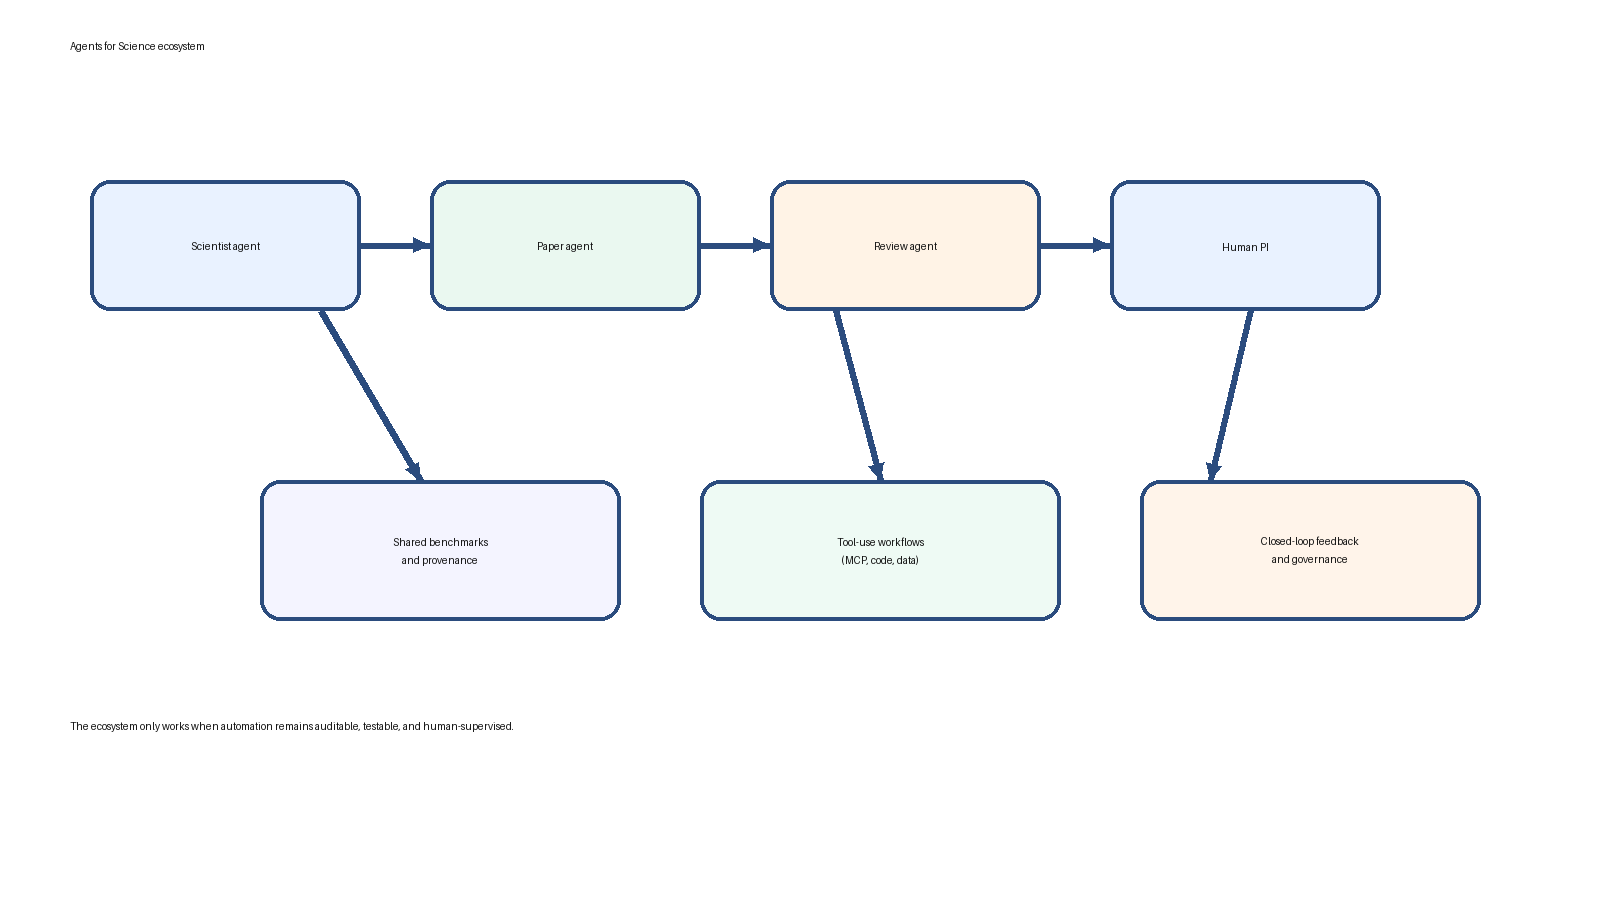
\includegraphics[width=0.94\linewidth]{figures/agentic_ecosystem.png}
  \caption{Agentic science ecosystem 的直观图景：paper agent、review agent、scientist agent 与人类研究者共同构成协作网络。}
\end{figure}

但课程同样强调了边界。第一，agent 仍然会 hallucinate，尤其是在长链路科研任务里。第二，很多研究工具并不是一开始就适合直接被“灌进模型”，因为文档、代码和数据结构可能过于复杂。第三，科学本身需要真实的闭环验证，不能只靠语言模型自说自话。Paper2Agent 对这些问题的回应不是回到纯手工，而是通过测试、迭代和工具封装把风险局部化。

\section{从 Virtual Lab 到 Agents for Science 的生态}
课程最后把视野放宽到一个更大的生态系统：Agents for Science。这里的意思不是单个论文，而是一个正在成形的研究共同体，包括自动科研、论文评审 agent、科学问答 agent、实验规划 agent 和人机协作工作流。课程视频提到，相关领域已经开始组织专门会议，说明这是一个快速增长的研究方向，而不是单点 demo。

在这个生态里，最关键的设计原则不是“放开自动化”，而是“逐步提升自主性”。合理的路径通常是：
\begin{itemize}[leftmargin=1.4em]
  \item 先让 agent 做文献检索、总结和工具调用。
  \item 再让它做局部实验设计、候选筛选和结果分析。
  \item 再通过专项 benchmark 和人类反馈校准它的可靠性。
  \item 最后才讨论更高程度的自治和跨 agent 协作。
\end{itemize}

\section{源缺口说明}
这一讲没有官方 slide PDF。讲义因此采用了视频字幕、课程页以及两篇官方 readings 作为主来源，并用自绘结构图补足教学表达。这个缺口是公开资源层面的事实，不是讲义写作失败；它只意味着这章的可视化更依赖教材化重构，而不是逐页复刻 slides。

\subsection{本章小结}
这一讲的核心结论很明确：AI agents 在科学发现中的价值，不在于替代研究者，而在于把科学流程拆成可交互、可审计、可复用的模块。Virtual Lab 说明了多 agent 分工如何嵌入科学组织；nanobody case study 说明了 agent 真的可以进入实验闭环；Paper2Agent 则进一步说明论文本身也可以成为 agent 的载体。三者合起来，构成了“科学知识从静态对象变成动态系统”的路线图。

\section{总结与延伸}
如果把这一讲和前两讲放在一起，就会发现一个共同结构：无论是多智能体博弈、评测噪声还是科学发现，真正重要的都不是单点模型能力，而是交互结构、反馈回路和制度化协作。Agentic AI 最有前景的方向，正是把这些结构变成可工程化、可复现、可审计的系统。

后续如果继续深入，最值得扩展的方向有两个：一是如何设计更可靠的 paper agents，让它们在不牺牲 provenance 的前提下支持自然语言查询；二是如何把实验室里的多智能体协作规范化为更通用的科学工作流。前者解决“怎么用”，后者解决“怎么扩展”。

\end{document}
